\documentclass[twoside]{book}

% Packages required by doxygen
\usepackage{fixltx2e}
\usepackage{calc}
\usepackage{doxygen}
\usepackage[export]{adjustbox} % also loads graphicx
\usepackage{graphicx}
\usepackage[utf8]{inputenc}
\usepackage{makeidx}
\usepackage{multicol}
\usepackage{multirow}
\PassOptionsToPackage{warn}{textcomp}
\usepackage{textcomp}
\usepackage[nointegrals]{wasysym}
\usepackage[table]{xcolor}

% Font selection
\usepackage[T1]{fontenc}
\usepackage[scaled=.90]{helvet}
\usepackage{courier}
\usepackage{amssymb}
\usepackage{sectsty}
\renewcommand{\familydefault}{\sfdefault}
\allsectionsfont{%
  \fontseries{bc}\selectfont%
  \color{darkgray}%
}
\renewcommand{\DoxyLabelFont}{%
  \fontseries{bc}\selectfont%
  \color{darkgray}%
}
\newcommand{\+}{\discretionary{\mbox{\scriptsize$\hookleftarrow$}}{}{}}

% Page & text layout
\usepackage{geometry}
\geometry{%
  a4paper,%
  top=2.5cm,%
  bottom=2.5cm,%
  left=2.5cm,%
  right=2.5cm%
}
\tolerance=750
\hfuzz=15pt
\hbadness=750
\setlength{\emergencystretch}{15pt}
\setlength{\parindent}{0cm}
\setlength{\parskip}{3ex plus 2ex minus 2ex}
\makeatletter
\renewcommand{\paragraph}{%
  \@startsection{paragraph}{4}{0ex}{-1.0ex}{1.0ex}{%
    \normalfont\normalsize\bfseries\SS@parafont%
  }%
}
\renewcommand{\subparagraph}{%
  \@startsection{subparagraph}{5}{0ex}{-1.0ex}{1.0ex}{%
    \normalfont\normalsize\bfseries\SS@subparafont%
  }%
}
\makeatother

% Headers & footers
\usepackage{fancyhdr}
\pagestyle{fancyplain}
\fancyhead[LE]{\fancyplain{}{\bfseries\thepage}}
\fancyhead[CE]{\fancyplain{}{}}
\fancyhead[RE]{\fancyplain{}{\bfseries\leftmark}}
\fancyhead[LO]{\fancyplain{}{\bfseries\rightmark}}
\fancyhead[CO]{\fancyplain{}{}}
\fancyhead[RO]{\fancyplain{}{\bfseries\thepage}}
\fancyfoot[LE]{\fancyplain{}{}}
\fancyfoot[CE]{\fancyplain{}{}}
\fancyfoot[RE]{\fancyplain{}{\bfseries\scriptsize Generated by Doxygen }}
\fancyfoot[LO]{\fancyplain{}{\bfseries\scriptsize Generated by Doxygen }}
\fancyfoot[CO]{\fancyplain{}{}}
\fancyfoot[RO]{\fancyplain{}{}}
\renewcommand{\footrulewidth}{0.4pt}
\renewcommand{\chaptermark}[1]{%
  \markboth{#1}{}%
}
\renewcommand{\sectionmark}[1]{%
  \markright{\thesection\ #1}%
}

% Indices & bibliography
\usepackage{natbib}
\usepackage[titles]{tocloft}
\setcounter{tocdepth}{3}
\setcounter{secnumdepth}{5}
\makeindex

% Hyperlinks (required, but should be loaded last)
\usepackage{ifpdf}
\ifpdf
  \usepackage[pdftex,pagebackref=true]{hyperref}
\else
  \usepackage[ps2pdf,pagebackref=true]{hyperref}
\fi
\hypersetup{%
  colorlinks=true,%
  linkcolor=blue,%
  citecolor=blue,%
  unicode%
}

% Custom commands
\newcommand{\clearemptydoublepage}{%
  \newpage{\pagestyle{empty}\cleardoublepage}%
}

\usepackage{caption}
\captionsetup{labelsep=space,justification=centering,font={bf},singlelinecheck=off,skip=4pt,position=top}

%===== C O N T E N T S =====

\begin{document}

% Titlepage & ToC
\hypersetup{pageanchor=false,
             bookmarksnumbered=true,
             pdfencoding=unicode
            }
\pagenumbering{alph}
\begin{titlepage}
\vspace*{7cm}
\begin{center}%
{\Large My Project }\\
\vspace*{1cm}
{\large Generated by Doxygen 1.8.13}\\
\end{center}
\end{titlepage}
\clearemptydoublepage
\pagenumbering{roman}
\tableofcontents
\clearemptydoublepage
\pagenumbering{arabic}
\hypersetup{pageanchor=true}

%--- Begin generated contents ---
\chapter{Hierarchical Index}
\section{Class Hierarchy}
This inheritance list is sorted roughly, but not completely, alphabetically\+:\begin{DoxyCompactList}
\item Mono\+Behaviour\begin{DoxyCompactList}
\item \contentsline{section}{Bullet}{\pageref{class_bullet}}{}
\item \contentsline{section}{Collisions}{\pageref{class_collisions}}{}
\item \contentsline{section}{Enemy\+Life}{\pageref{class_enemy_life}}{}
\item \contentsline{section}{Generating\+Enemies}{\pageref{class_generating_enemies}}{}
\item \contentsline{section}{Level\+Script}{\pageref{class_level_script}}{}
\item \contentsline{section}{Movement}{\pageref{class_movement}}{}
\item \contentsline{section}{Pumpkin\+Click}{\pageref{class_pumpkin_click}}{}
\item \contentsline{section}{Pumpkin\+Collisions}{\pageref{class_pumpkin_collisions}}{}
\item \contentsline{section}{Pumpkin\+Manager}{\pageref{class_pumpkin_manager}}{}
\item \contentsline{section}{Pumpkin\+Selection}{\pageref{class_pumpkin_selection}}{}
\item \contentsline{section}{Rotate}{\pageref{class_rotate}}{}
\item \contentsline{section}{Score\+Script}{\pageref{class_score_script}}{}
\item \contentsline{section}{Singleton$<$ T $>$}{\pageref{class_singleton}}{}
\item \contentsline{section}{You\+Loose}{\pageref{class_you_loose}}{}
\end{DoxyCompactList}
\item \contentsline{section}{Point}{\pageref{struct_point}}{}
\item \contentsline{section}{Pumpkin}{\pageref{class_pumpkin}}{}
\item \contentsline{section}{Singleton$<$ Hover $>$}{\pageref{class_singleton}}{}
\begin{DoxyCompactList}
\item \contentsline{section}{Hover}{\pageref{class_hover}}{}
\end{DoxyCompactList}
\end{DoxyCompactList}

\chapter{Class Index}
\section{Class List}
Here are the classes, structs, unions and interfaces with brief descriptions\+:\begin{DoxyCompactList}
\item\contentsline{section}{\hyperlink{class_bullet}{Bullet} }{\pageref{class_bullet}}{}
\item\contentsline{section}{\hyperlink{class_collisions}{Collisions} }{\pageref{class_collisions}}{}
\item\contentsline{section}{\hyperlink{class_enemy_life}{Enemy\+Life} }{\pageref{class_enemy_life}}{}
\item\contentsline{section}{\hyperlink{class_generating_enemies}{Generating\+Enemies} }{\pageref{class_generating_enemies}}{}
\item\contentsline{section}{\hyperlink{class_hover}{Hover} }{\pageref{class_hover}}{}
\item\contentsline{section}{\hyperlink{class_level_script}{Level\+Script} }{\pageref{class_level_script}}{}
\item\contentsline{section}{\hyperlink{class_movement}{Movement} }{\pageref{class_movement}}{}
\item\contentsline{section}{\hyperlink{struct_point}{Point} }{\pageref{struct_point}}{}
\item\contentsline{section}{\hyperlink{class_pumpkin}{Pumpkin} }{\pageref{class_pumpkin}}{}
\item\contentsline{section}{\hyperlink{class_pumpkin_click}{Pumpkin\+Click} }{\pageref{class_pumpkin_click}}{}
\item\contentsline{section}{\hyperlink{class_pumpkin_collisions}{Pumpkin\+Collisions} }{\pageref{class_pumpkin_collisions}}{}
\item\contentsline{section}{\hyperlink{class_pumpkin_manager}{Pumpkin\+Manager} }{\pageref{class_pumpkin_manager}}{}
\item\contentsline{section}{\hyperlink{class_pumpkin_selection}{Pumpkin\+Selection} }{\pageref{class_pumpkin_selection}}{}
\item\contentsline{section}{\hyperlink{class_rotate}{Rotate} }{\pageref{class_rotate}}{}
\item\contentsline{section}{\hyperlink{class_score_script}{Score\+Script} }{\pageref{class_score_script}}{}
\item\contentsline{section}{\hyperlink{class_singleton}{Singleton$<$ T $>$} \\*Be aware this will not prevent a non singleton constructor such as {\ttfamily T myT = new T();} To prevent that, add {\ttfamily protected T () \{\}} to your singleton class }{\pageref{class_singleton}}{}
\item\contentsline{section}{\hyperlink{class_you_loose}{You\+Loose} }{\pageref{class_you_loose}}{}
\end{DoxyCompactList}

\chapter{Class Documentation}
\hypertarget{class_bullet}{}\section{Bullet Class Reference}
\label{class_bullet}\index{Bullet@{Bullet}}
Inheritance diagram for Bullet\+:\begin{figure}[H]
\begin{center}
\leavevmode
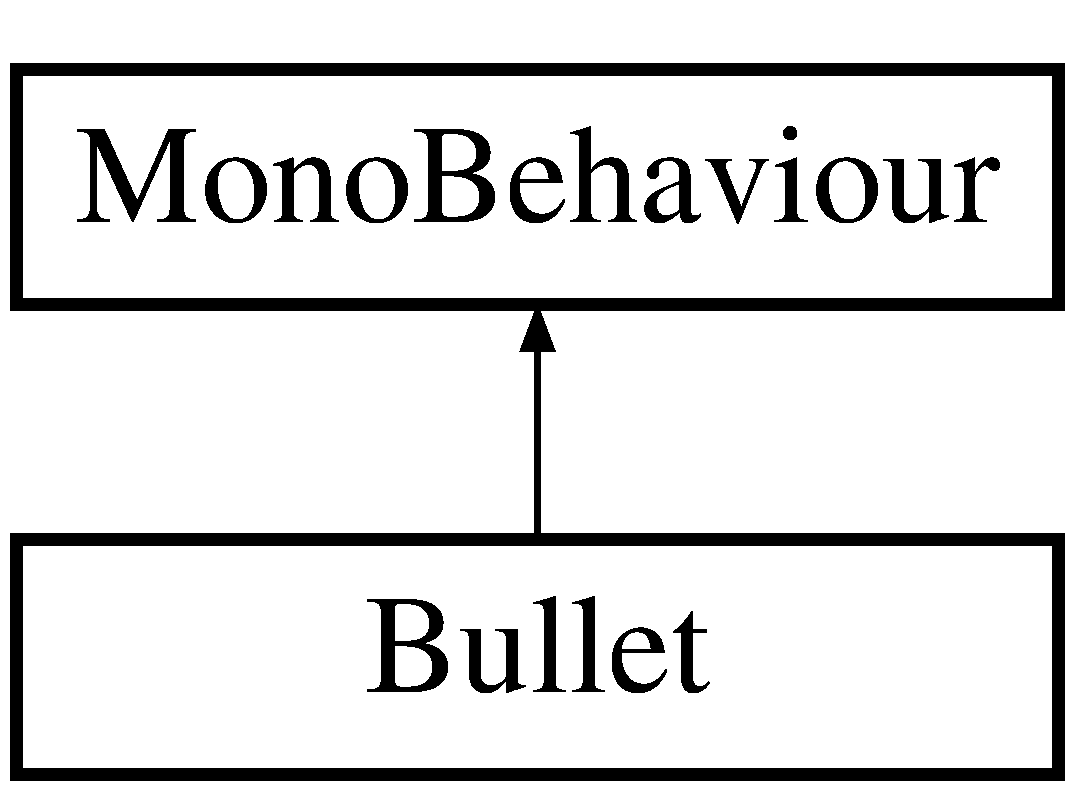
\includegraphics[height=2.000000cm]{class_bullet}
\end{center}
\end{figure}
\subsection*{Public Attributes}
\begin{DoxyCompactItemize}
\item 
Game\+Object \hyperlink{class_bullet_ace755c0a98317cf6aefa1d69949081cf}{bullet\+Prefab}
\item 
float \hyperlink{class_bullet_a75e914c39a4154ced3d653ae44a05539}{speed}
\item 
float \hyperlink{class_bullet_ae35c2a21d9d6abff09869e1a9f3b2053}{time}
\end{DoxyCompactItemize}


\subsection{Detailed Description}
Generare de proiectile 

\subsection{Member Data Documentation}
\mbox{\Hypertarget{class_bullet_ace755c0a98317cf6aefa1d69949081cf}\label{class_bullet_ace755c0a98317cf6aefa1d69949081cf}} 
\index{Bullet@{Bullet}!bullet\+Prefab@{bullet\+Prefab}}
\index{bullet\+Prefab@{bullet\+Prefab}!Bullet@{Bullet}}
\subsubsection{\texorpdfstring{bullet\+Prefab}{bulletPrefab}}
{\footnotesize\ttfamily Game\+Object Bullet.\+bullet\+Prefab}

Tipul de proiectil \mbox{\Hypertarget{class_bullet_a75e914c39a4154ced3d653ae44a05539}\label{class_bullet_a75e914c39a4154ced3d653ae44a05539}} 
\index{Bullet@{Bullet}!speed@{speed}}
\index{speed@{speed}!Bullet@{Bullet}}
\subsubsection{\texorpdfstring{speed}{speed}}
{\footnotesize\ttfamily float Bullet.\+speed}

Viteza proiectulului \mbox{\Hypertarget{class_bullet_ae35c2a21d9d6abff09869e1a9f3b2053}\label{class_bullet_ae35c2a21d9d6abff09869e1a9f3b2053}} 
\index{Bullet@{Bullet}!time@{time}}
\index{time@{time}!Bullet@{Bullet}}
\subsubsection{\texorpdfstring{time}{time}}
{\footnotesize\ttfamily float Bullet.\+time}

Timpul la care este lansat 

The documentation for this class was generated from the following file\+:\begin{DoxyCompactItemize}
\item 
Halloween\+Attack/\+Assets/halloween\+Attack/\+Scripts/Bullet.\+cs\end{DoxyCompactItemize}

\hypertarget{class_collisions}{}\section{Collisions Class Reference}
\label{class_collisions}\index{Collisions@{Collisions}}
Inheritance diagram for Collisions\+:\begin{figure}[H]
\begin{center}
\leavevmode
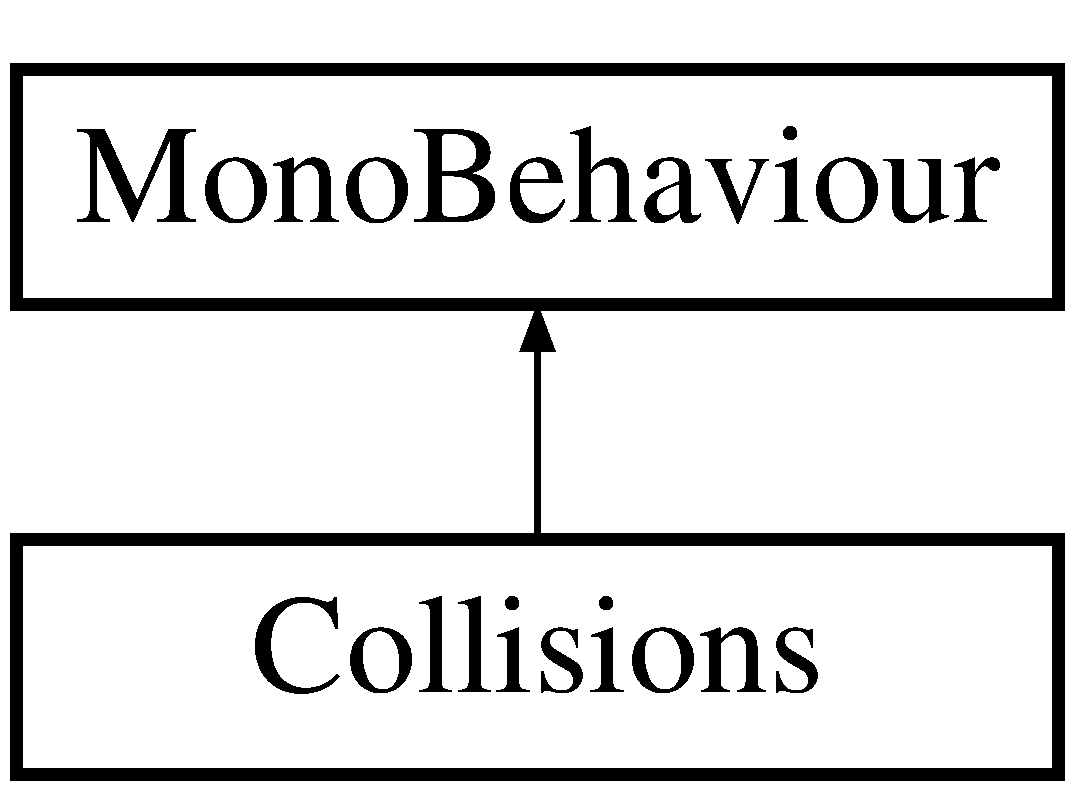
\includegraphics[height=2.000000cm]{class_collisions}
\end{center}
\end{figure}


\subsection{Detailed Description}
Se ocupa cu controlul coliziunilor inamicilor cu dovlecii 

The documentation for this class was generated from the following file\+:\begin{DoxyCompactItemize}
\item 
Halloween\+Attack/\+Assets/halloween\+Attack/\+Scripts/Collisions.\+cs\end{DoxyCompactItemize}

\hypertarget{class_enemy_life}{}\section{Enemy\+Life Class Reference}
\label{class_enemy_life}\index{Enemy\+Life@{Enemy\+Life}}
Inheritance diagram for Enemy\+Life\+:\begin{figure}[H]
\begin{center}
\leavevmode
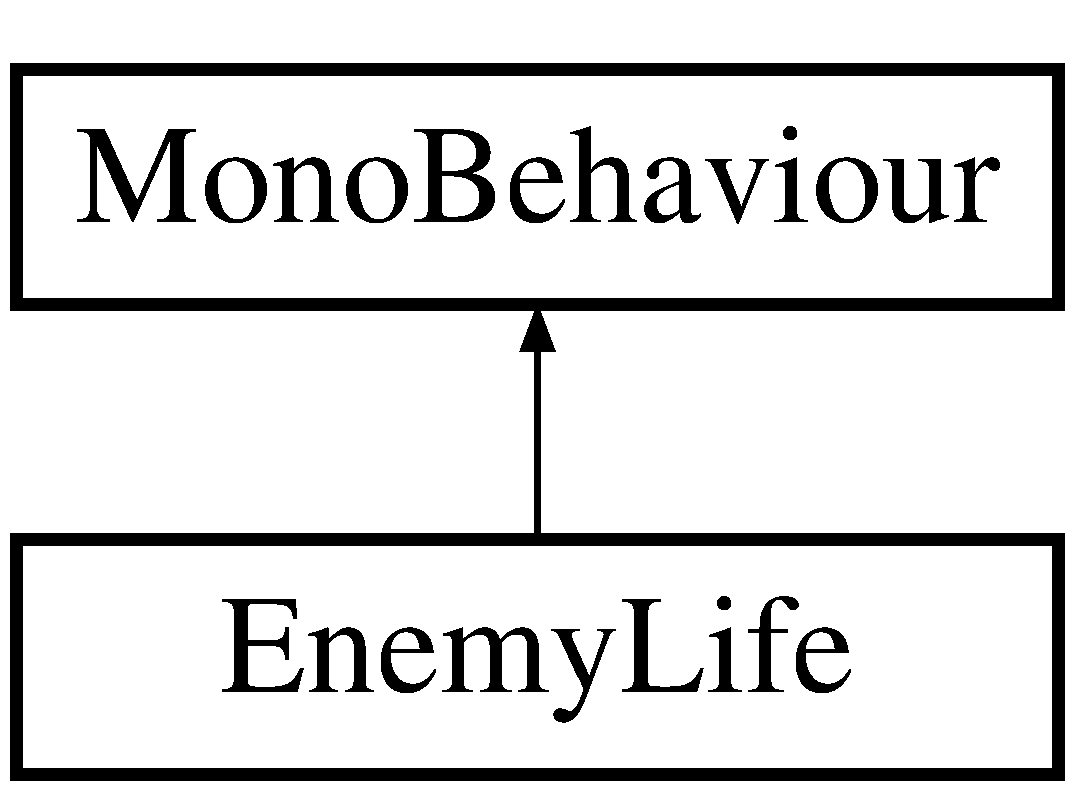
\includegraphics[height=2.000000cm]{class_enemy_life}
\end{center}
\end{figure}
\subsection*{Public Member Functions}
\begin{DoxyCompactItemize}
\item 
\mbox{\Hypertarget{class_enemy_life_a04184d58b33094d37f07c4a680f46915}\label{class_enemy_life_a04184d58b33094d37f07c4a680f46915}} 
int {\bfseries get\+Points} ()
\end{DoxyCompactItemize}
\subsection*{Public Attributes}
\begin{DoxyCompactItemize}
\item 
int \hyperlink{class_enemy_life_a1a9366e42605193f61910a80ed0d177e}{life}
\end{DoxyCompactItemize}


\subsection{Detailed Description}
Gestioneaza nivelul vietii inamicului 

\subsection{Member Data Documentation}
\mbox{\Hypertarget{class_enemy_life_a1a9366e42605193f61910a80ed0d177e}\label{class_enemy_life_a1a9366e42605193f61910a80ed0d177e}} 
\index{Enemy\+Life@{Enemy\+Life}!life@{life}}
\index{life@{life}!Enemy\+Life@{Enemy\+Life}}
\subsubsection{\texorpdfstring{life}{life}}
{\footnotesize\ttfamily int Enemy\+Life.\+life}

Nivelul vietii 

The documentation for this class was generated from the following file\+:\begin{DoxyCompactItemize}
\item 
Halloween\+Attack/\+Assets/halloween\+Attack/\+Scripts/Enemy\+Life.\+cs\end{DoxyCompactItemize}

\hypertarget{class_generating_enemies}{}\section{Generating\+Enemies Class Reference}
\label{class_generating_enemies}\index{Generating\+Enemies@{Generating\+Enemies}}
Inheritance diagram for Generating\+Enemies\+:\begin{figure}[H]
\begin{center}
\leavevmode
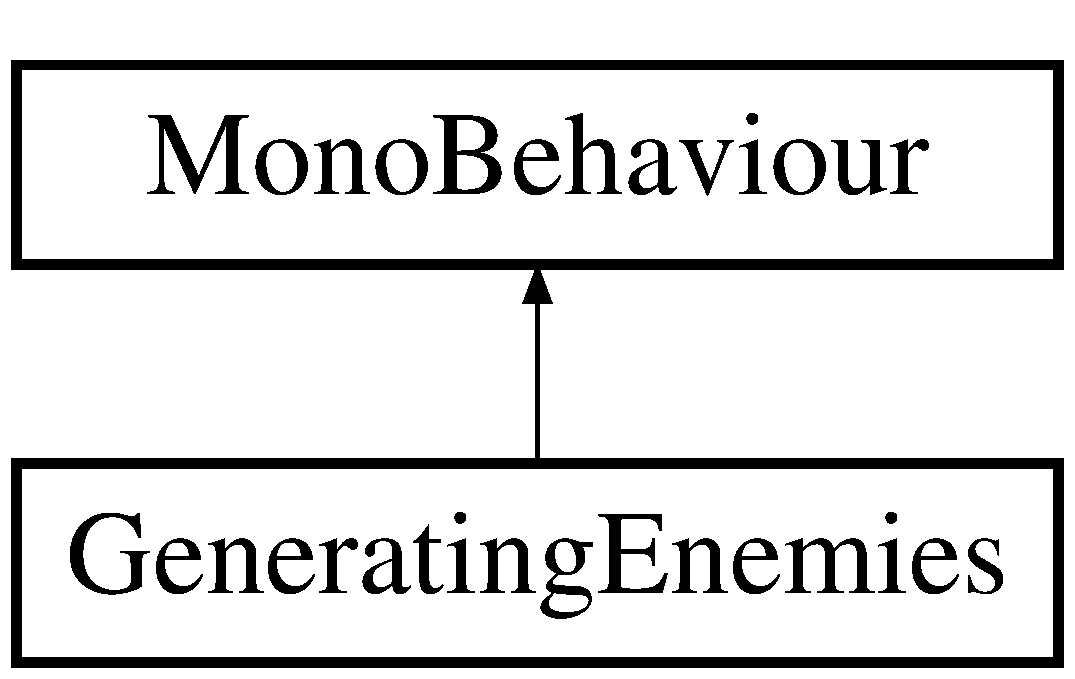
\includegraphics[height=2.000000cm]{class_generating_enemies}
\end{center}
\end{figure}
\subsection*{Public Attributes}
\begin{DoxyCompactItemize}
\item 
Game\+Object \hyperlink{class_generating_enemies_ad1010803ac8fc15527679c7d6e544397}{prefab}
\item 
float \hyperlink{class_generating_enemies_a6e62912d45be356c13984ef19569879a}{time}
\end{DoxyCompactItemize}


\subsection{Detailed Description}
Genereaza inamici in functie de nivel 

\subsection{Member Data Documentation}
\mbox{\Hypertarget{class_generating_enemies_ad1010803ac8fc15527679c7d6e544397}\label{class_generating_enemies_ad1010803ac8fc15527679c7d6e544397}} 
\index{Generating\+Enemies@{Generating\+Enemies}!prefab@{prefab}}
\index{prefab@{prefab}!Generating\+Enemies@{Generating\+Enemies}}
\subsubsection{\texorpdfstring{prefab}{prefab}}
{\footnotesize\ttfamily Game\+Object Generating\+Enemies.\+prefab}

tipul de inamic \mbox{\Hypertarget{class_generating_enemies_a6e62912d45be356c13984ef19569879a}\label{class_generating_enemies_a6e62912d45be356c13984ef19569879a}} 
\index{Generating\+Enemies@{Generating\+Enemies}!time@{time}}
\index{time@{time}!Generating\+Enemies@{Generating\+Enemies}}
\subsubsection{\texorpdfstring{time}{time}}
{\footnotesize\ttfamily float Generating\+Enemies.\+time}

timpul dupa care se genereaza 

The documentation for this class was generated from the following file\+:\begin{DoxyCompactItemize}
\item 
Halloween\+Attack/\+Assets/halloween\+Attack/\+Scripts/Generating\+Enemies.\+cs\end{DoxyCompactItemize}

\hypertarget{class_hover}{}\section{Hover Class Reference}
\label{class_hover}\index{Hover@{Hover}}
Inheritance diagram for Hover\+:\begin{figure}[H]
\begin{center}
\leavevmode
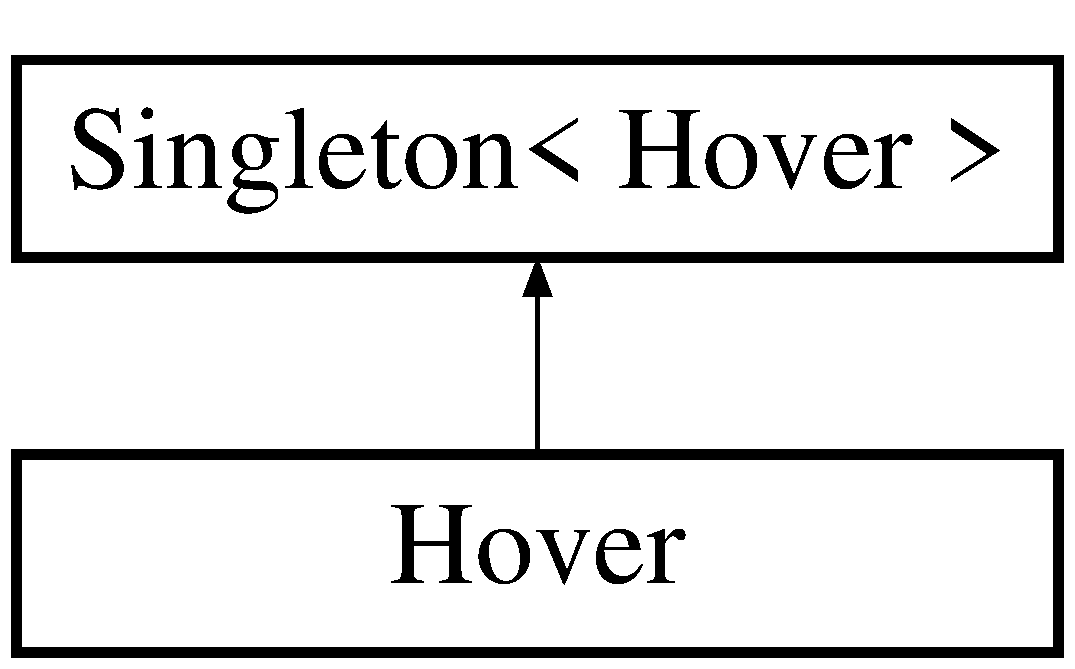
\includegraphics[height=2.000000cm]{class_hover}
\end{center}
\end{figure}
\subsection*{Public Member Functions}
\begin{DoxyCompactItemize}
\item 
\mbox{\Hypertarget{class_hover_a04c0b6d29a85d5f8ae51eaba6fc11cd0}\label{class_hover_a04c0b6d29a85d5f8ae51eaba6fc11cd0}} 
void {\bfseries Activate} (Sprite sprite)
\item 
\mbox{\Hypertarget{class_hover_aae6c1f16666c7574857cf6d74c700bbb}\label{class_hover_aae6c1f16666c7574857cf6d74c700bbb}} 
void {\bfseries Deactivate} ()
\end{DoxyCompactItemize}
\subsection*{Public Attributes}
\begin{DoxyCompactItemize}
\item 
\mbox{\Hypertarget{class_hover_a38509a892cf15f821d95403bfce8a7dc}\label{class_hover_a38509a892cf15f821d95403bfce8a7dc}} 
Sprite\+Renderer {\bfseries sprite\+Renderer}
\end{DoxyCompactItemize}
\subsection*{Additional Inherited Members}


\subsection{Detailed Description}
Controleaza miscarea dovleacului dupa mouse pana la plasarea pe harta 

The documentation for this class was generated from the following file\+:\begin{DoxyCompactItemize}
\item 
Halloween\+Attack/\+Assets/halloween\+Attack/\+Scripts/Hover.\+cs\end{DoxyCompactItemize}

\hypertarget{class_level_script}{}\section{Level\+Script Class Reference}
\label{class_level_script}\index{Level\+Script@{Level\+Script}}
Inheritance diagram for Level\+Script\+:\begin{figure}[H]
\begin{center}
\leavevmode
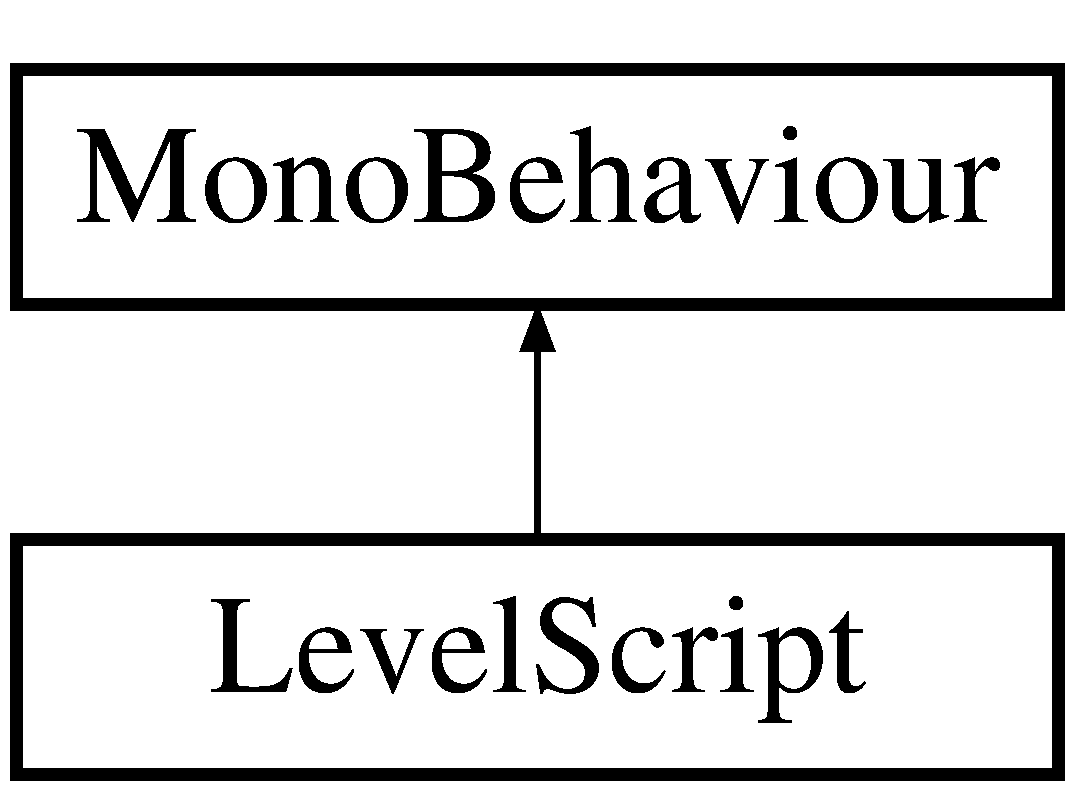
\includegraphics[height=2.000000cm]{class_level_script}
\end{center}
\end{figure}
\subsection*{Static Public Attributes}
\begin{DoxyCompactItemize}
\item 
static string \hyperlink{class_level_script_abb5aff606d2a904687daa65de8807278}{level\+Value} = \char`\"{}1\char`\"{}
\end{DoxyCompactItemize}


\subsection{Detailed Description}
Gestioneaza numarul nivelului curent 

\subsection{Member Data Documentation}
\mbox{\Hypertarget{class_level_script_abb5aff606d2a904687daa65de8807278}\label{class_level_script_abb5aff606d2a904687daa65de8807278}} 
\index{Level\+Script@{Level\+Script}!level\+Value@{level\+Value}}
\index{level\+Value@{level\+Value}!Level\+Script@{Level\+Script}}
\subsubsection{\texorpdfstring{level\+Value}{levelValue}}
{\footnotesize\ttfamily string Level\+Script.\+level\+Value = \char`\"{}1\char`\"{}\hspace{0.3cm}{\ttfamily [static]}}

Nivelul curent 

The documentation for this class was generated from the following file\+:\begin{DoxyCompactItemize}
\item 
Halloween\+Attack/\+Assets/halloween\+Attack/\+Scripts/Level\+Script.\+cs\end{DoxyCompactItemize}

\hypertarget{class_movement}{}\section{Movement Class Reference}
\label{class_movement}\index{Movement@{Movement}}
Inheritance diagram for Movement\+:\begin{figure}[H]
\begin{center}
\leavevmode
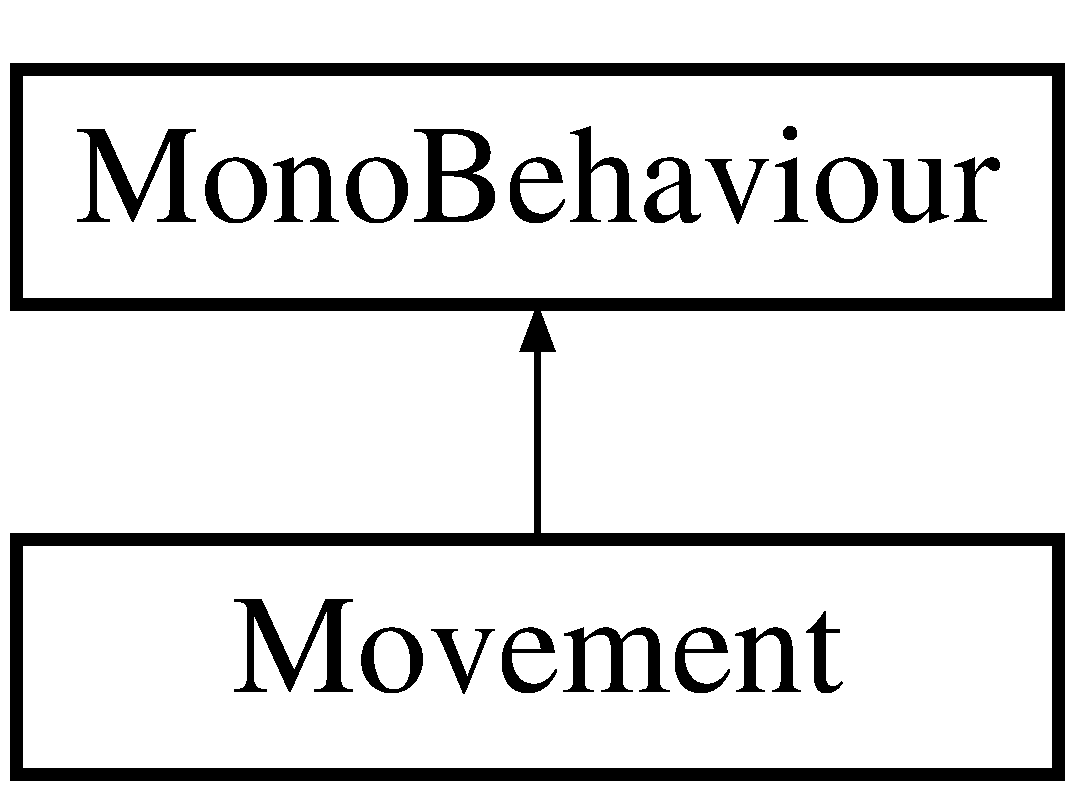
\includegraphics[height=2.000000cm]{class_movement}
\end{center}
\end{figure}
\subsection*{Public Attributes}
\begin{DoxyCompactItemize}
\item 
float \hyperlink{class_movement_aba07bc6bfeba07294bfd68dec4962388}{speed}
\end{DoxyCompactItemize}


\subsection{Detailed Description}
Gestioneaza miscarea inamicilor 

\subsection{Member Data Documentation}
\mbox{\Hypertarget{class_movement_aba07bc6bfeba07294bfd68dec4962388}\label{class_movement_aba07bc6bfeba07294bfd68dec4962388}} 
\index{Movement@{Movement}!speed@{speed}}
\index{speed@{speed}!Movement@{Movement}}
\subsubsection{\texorpdfstring{speed}{speed}}
{\footnotesize\ttfamily float Movement.\+speed}

Viteza cu care se deplaseaza inamicii 

The documentation for this class was generated from the following file\+:\begin{DoxyCompactItemize}
\item 
Halloween\+Attack/\+Assets/halloween\+Attack/\+Scripts/Movement.\+cs\end{DoxyCompactItemize}

\hypertarget{struct_point}{}\section{Point Struct Reference}
\label{struct_point}\index{Point@{Point}}
\subsection*{Public Member Functions}
\begin{DoxyCompactItemize}
\item 
\mbox{\Hypertarget{struct_point_a936b3f1136112cccf9719fb3b294b2b9}\label{struct_point_a936b3f1136112cccf9719fb3b294b2b9}} 
{\bfseries Point} (int x, int y)
\end{DoxyCompactItemize}
\subsection*{Static Public Member Functions}
\begin{DoxyCompactItemize}
\item 
\mbox{\Hypertarget{struct_point_a9f41928a50d8c3df7701df79f90fab91}\label{struct_point_a9f41928a50d8c3df7701df79f90fab91}} 
static bool {\bfseries operator==} (\hyperlink{struct_point}{Point} p1, \hyperlink{struct_point}{Point} p2)
\item 
\mbox{\Hypertarget{struct_point_a2d4f94967363875413d1d709afd8f755}\label{struct_point_a2d4f94967363875413d1d709afd8f755}} 
static bool {\bfseries operator!=} (\hyperlink{struct_point}{Point} p1, \hyperlink{struct_point}{Point} p2)
\end{DoxyCompactItemize}
\subsection*{Properties}
\begin{DoxyCompactItemize}
\item 
int \hyperlink{struct_point_a944eb35c3d0b0efea5555a82a8c4a6fc}{X}\hspace{0.3cm}{\ttfamily  \mbox{[}get, set\mbox{]}}
\item 
int \hyperlink{struct_point_ac41b750e0b7eb2adbe2c808e4521a94b}{Y}\hspace{0.3cm}{\ttfamily  \mbox{[}get, set\mbox{]}}
\end{DoxyCompactItemize}


\subsection{Detailed Description}
Retine coordonatele de pe harta si permite operatii primitive cu acestea 

\subsection{Property Documentation}
\mbox{\Hypertarget{struct_point_a944eb35c3d0b0efea5555a82a8c4a6fc}\label{struct_point_a944eb35c3d0b0efea5555a82a8c4a6fc}} 
\index{Point@{Point}!X@{X}}
\index{X@{X}!Point@{Point}}
\subsubsection{\texorpdfstring{X}{X}}
{\footnotesize\ttfamily int Point.\+X\hspace{0.3cm}{\ttfamily [get]}, {\ttfamily [set]}}

Coordonata X \mbox{\Hypertarget{struct_point_ac41b750e0b7eb2adbe2c808e4521a94b}\label{struct_point_ac41b750e0b7eb2adbe2c808e4521a94b}} 
\index{Point@{Point}!Y@{Y}}
\index{Y@{Y}!Point@{Point}}
\subsubsection{\texorpdfstring{Y}{Y}}
{\footnotesize\ttfamily int Point.\+Y\hspace{0.3cm}{\ttfamily [get]}, {\ttfamily [set]}}

Coordonata Y 

The documentation for this struct was generated from the following file\+:\begin{DoxyCompactItemize}
\item 
Halloween\+Attack/\+Assets/halloween\+Attack/\+Scripts/Point.\+cs\end{DoxyCompactItemize}

\hypertarget{class_pumpkin}{}\section{Pumpkin Class Reference}
\label{class_pumpkin}\index{Pumpkin@{Pumpkin}}
\subsection*{Public Member Functions}
\begin{DoxyCompactItemize}
\item 
\mbox{\Hypertarget{class_pumpkin_ad48994bb743f7547b17516a3599808da}\label{class_pumpkin_ad48994bb743f7547b17516a3599808da}} 
{\bfseries Pumpkin} (\hyperlink{struct_point}{Point} p)
\item 
\mbox{\Hypertarget{class_pumpkin_aef1982c1ef62d3f74fcc345a03a7f54f}\label{class_pumpkin_aef1982c1ef62d3f74fcc345a03a7f54f}} 
void {\bfseries move\+Up} ()
\item 
\mbox{\Hypertarget{class_pumpkin_a3afb056b649203f4c49171f598d1711a}\label{class_pumpkin_a3afb056b649203f4c49171f598d1711a}} 
void {\bfseries move\+Down} ()
\item 
\mbox{\Hypertarget{class_pumpkin_ab8228ef139ace9c450d4d936e5e2a500}\label{class_pumpkin_ab8228ef139ace9c450d4d936e5e2a500}} 
void {\bfseries move\+Left} ()
\item 
\mbox{\Hypertarget{class_pumpkin_abc72185ad960e4c54658b7826faf79ce}\label{class_pumpkin_abc72185ad960e4c54658b7826faf79ce}} 
void {\bfseries move\+Right} ()
\end{DoxyCompactItemize}
\subsection*{Public Attributes}
\begin{DoxyCompactItemize}
\item 
\mbox{\Hypertarget{class_pumpkin_aa2ab337ccbb0855810684bdc68d55146}\label{class_pumpkin_aa2ab337ccbb0855810684bdc68d55146}} 
Sprite\+Renderer {\bfseries sprite\+Renderer}
\end{DoxyCompactItemize}
\subsection*{Properties}
\begin{DoxyCompactItemize}
\item 
\hyperlink{struct_point}{Point} \hyperlink{class_pumpkin_aa958881a119da828858daf9e3bc069de}{Grid\+Position}\hspace{0.3cm}{\ttfamily  \mbox{[}get, set\mbox{]}}
\end{DoxyCompactItemize}


\subsection{Detailed Description}
Permite deplasarea dovleacului pana la amplasare 

\subsection{Property Documentation}
\mbox{\Hypertarget{class_pumpkin_aa958881a119da828858daf9e3bc069de}\label{class_pumpkin_aa958881a119da828858daf9e3bc069de}} 
\index{Pumpkin@{Pumpkin}!Grid\+Position@{Grid\+Position}}
\index{Grid\+Position@{Grid\+Position}!Pumpkin@{Pumpkin}}
\subsubsection{\texorpdfstring{Grid\+Position}{GridPosition}}
{\footnotesize\ttfamily \hyperlink{struct_point}{Point} Pumpkin.\+Grid\+Position\hspace{0.3cm}{\ttfamily [get]}, {\ttfamily [set]}}

Pozitie curenta 

The documentation for this class was generated from the following file\+:\begin{DoxyCompactItemize}
\item 
Halloween\+Attack/\+Assets/halloween\+Attack/\+Scripts/Pumpkin.\+cs\end{DoxyCompactItemize}

\hypertarget{class_pumpkin_click}{}\section{Pumpkin\+Click Class Reference}
\label{class_pumpkin_click}\index{Pumpkin\+Click@{Pumpkin\+Click}}
Inheritance diagram for Pumpkin\+Click\+:\begin{figure}[H]
\begin{center}
\leavevmode
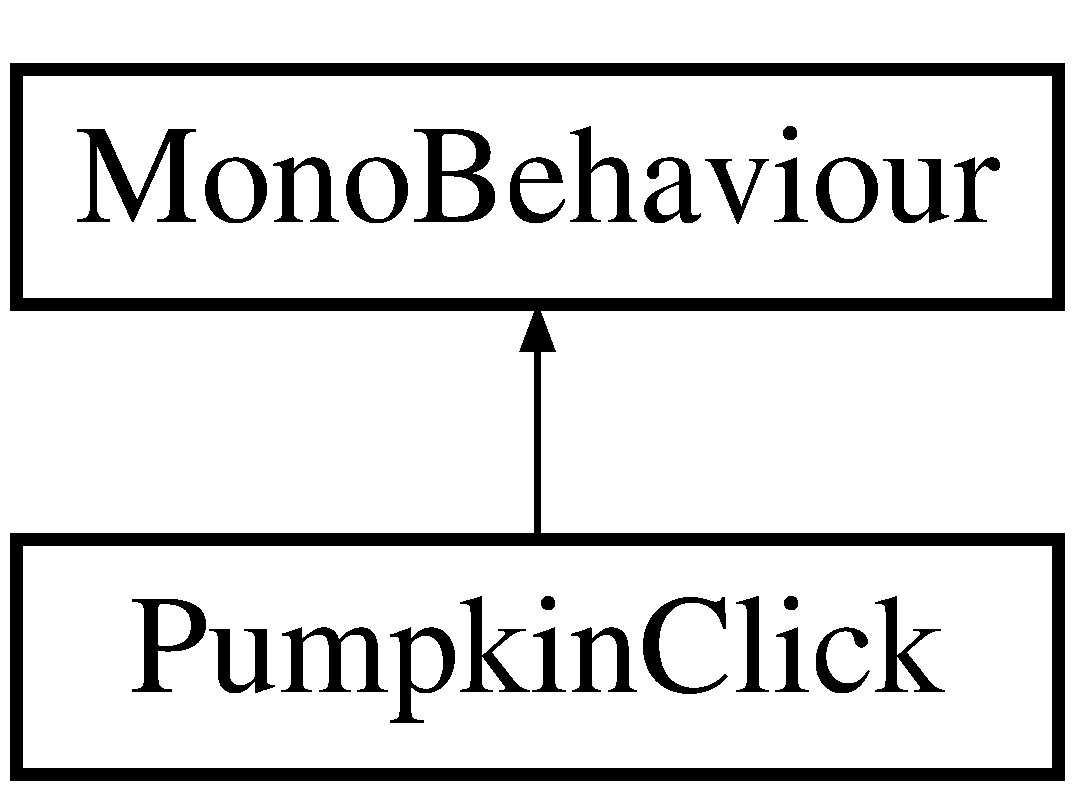
\includegraphics[height=2.000000cm]{class_pumpkin_click}
\end{center}
\end{figure}


\subsection{Detailed Description}
Se ocupa de upgradarea elementului defensiv 

The documentation for this class was generated from the following file\+:\begin{DoxyCompactItemize}
\item 
Halloween\+Attack/\+Assets/halloween\+Attack/\+Scripts/Pumpkin\+Click.\+cs\end{DoxyCompactItemize}

\hypertarget{class_pumpkin_collisions}{}\section{Pumpkin\+Collisions Class Reference}
\label{class_pumpkin_collisions}\index{Pumpkin\+Collisions@{Pumpkin\+Collisions}}
Inheritance diagram for Pumpkin\+Collisions\+:\begin{figure}[H]
\begin{center}
\leavevmode
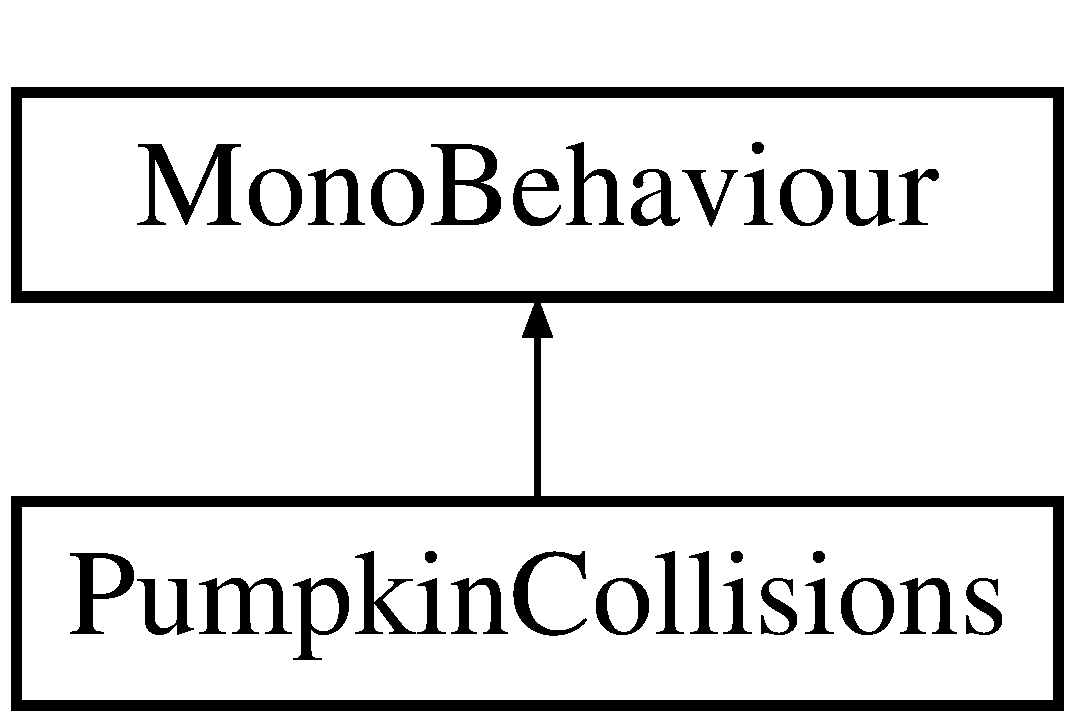
\includegraphics[height=2.000000cm]{class_pumpkin_collisions}
\end{center}
\end{figure}


\subsection{Detailed Description}
Se ocupa de coliziunile elementelor defensive cu inamicii si proiectilele acestora 

The documentation for this class was generated from the following file\+:\begin{DoxyCompactItemize}
\item 
Halloween\+Attack/\+Assets/halloween\+Attack/\+Scripts/Pumpkin\+Collisions.\+cs\end{DoxyCompactItemize}

\hypertarget{class_pumpkin_manager}{}\section{Pumpkin\+Manager Class Reference}
\label{class_pumpkin_manager}\index{Pumpkin\+Manager@{Pumpkin\+Manager}}
Inheritance diagram for Pumpkin\+Manager\+:\begin{figure}[H]
\begin{center}
\leavevmode
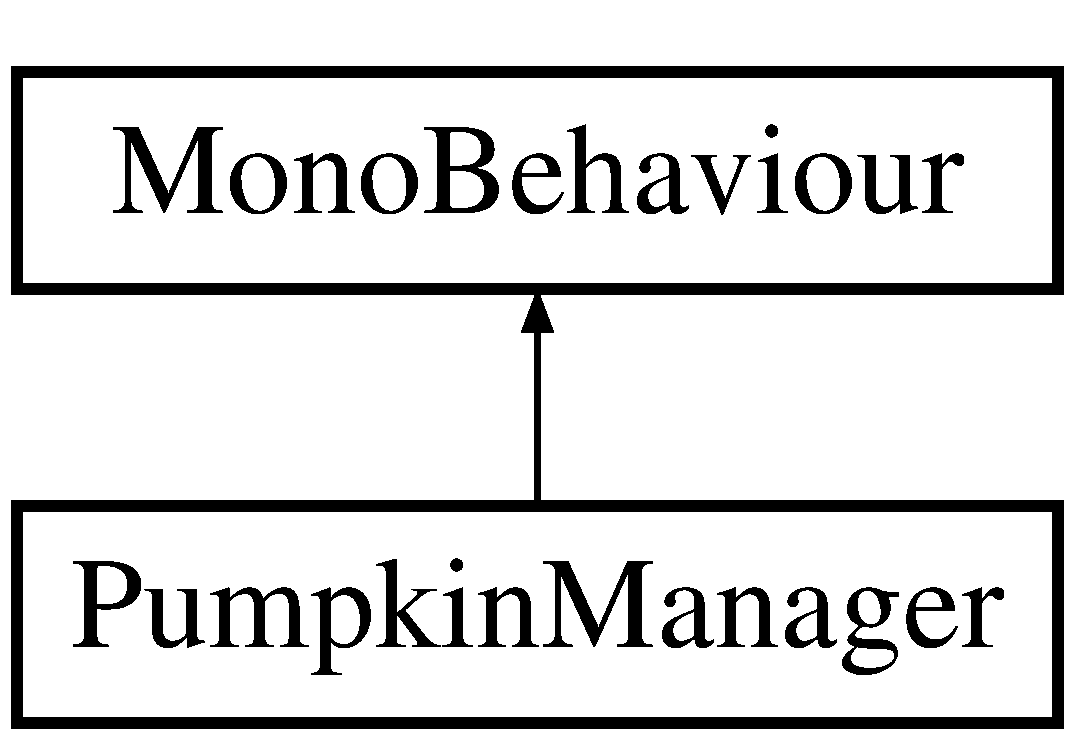
\includegraphics[height=2.000000cm]{class_pumpkin_manager}
\end{center}
\end{figure}
\subsection*{Public Member Functions}
\begin{DoxyCompactItemize}
\item 
\mbox{\Hypertarget{class_pumpkin_manager_a632fd636607c8067c0ebd5cdf747ccf2}\label{class_pumpkin_manager_a632fd636607c8067c0ebd5cdf747ccf2}} 
void {\bfseries Pick\+Pumpkin} (\hyperlink{class_pumpkin_selection}{Pumpkin\+Selection} selection)
\item 
\mbox{\Hypertarget{class_pumpkin_manager_ab71217876313a82259997c561979126c}\label{class_pumpkin_manager_ab71217876313a82259997c561979126c}} 
int {\bfseries Buy\+Pumpkin} (Game\+Object pumpkin)
\end{DoxyCompactItemize}
\subsection*{Public Attributes}
\begin{DoxyCompactItemize}
\item 
Game\+Object \hyperlink{class_pumpkin_manager_aa64ea8a9e81650b43409b291f9bd5e20}{p1\+Selection}
\item 
\hyperlink{class_pumpkin_selection}{Pumpkin\+Selection} \hyperlink{class_pumpkin_manager_ab4437ea939dfb4ec5c00c35b7962209c}{clicked\+Selection}
\end{DoxyCompactItemize}
\subsection*{Static Public Attributes}
\begin{DoxyCompactItemize}
\item 
static int \hyperlink{class_pumpkin_manager_a4286037e6502dd8f5b9d9ef22b513bb9}{has\+Money}
\end{DoxyCompactItemize}


\subsection{Detailed Description}
Coordoneaza tot procesul de amplasare a unui dovleac pe harta, inclusiv costul acestuia 

\subsection{Member Data Documentation}
\mbox{\Hypertarget{class_pumpkin_manager_ab4437ea939dfb4ec5c00c35b7962209c}\label{class_pumpkin_manager_ab4437ea939dfb4ec5c00c35b7962209c}} 
\index{Pumpkin\+Manager@{Pumpkin\+Manager}!clicked\+Selection@{clicked\+Selection}}
\index{clicked\+Selection@{clicked\+Selection}!Pumpkin\+Manager@{Pumpkin\+Manager}}
\subsubsection{\texorpdfstring{clicked\+Selection}{clickedSelection}}
{\footnotesize\ttfamily \hyperlink{class_pumpkin_selection}{Pumpkin\+Selection} Pumpkin\+Manager.\+clicked\+Selection}

Dovleacul selectat \mbox{\Hypertarget{class_pumpkin_manager_a4286037e6502dd8f5b9d9ef22b513bb9}\label{class_pumpkin_manager_a4286037e6502dd8f5b9d9ef22b513bb9}} 
\index{Pumpkin\+Manager@{Pumpkin\+Manager}!has\+Money@{has\+Money}}
\index{has\+Money@{has\+Money}!Pumpkin\+Manager@{Pumpkin\+Manager}}
\subsubsection{\texorpdfstring{has\+Money}{hasMoney}}
{\footnotesize\ttfamily int Pumpkin\+Manager.\+has\+Money\hspace{0.3cm}{\ttfamily [static]}}

Indica daca utilizatorul mai are destui bani pentru a cumpara dovleacul \mbox{\Hypertarget{class_pumpkin_manager_aa64ea8a9e81650b43409b291f9bd5e20}\label{class_pumpkin_manager_aa64ea8a9e81650b43409b291f9bd5e20}} 
\index{Pumpkin\+Manager@{Pumpkin\+Manager}!p1\+Selection@{p1\+Selection}}
\index{p1\+Selection@{p1\+Selection}!Pumpkin\+Manager@{Pumpkin\+Manager}}
\subsubsection{\texorpdfstring{p1\+Selection}{p1Selection}}
{\footnotesize\ttfamily Game\+Object Pumpkin\+Manager.\+p1\+Selection}

Cele 3 tipuri de dovleci 

The documentation for this class was generated from the following file\+:\begin{DoxyCompactItemize}
\item 
Halloween\+Attack/\+Assets/halloween\+Attack/\+Scripts/Pumpkin\+Manager.\+cs\end{DoxyCompactItemize}

\hypertarget{class_pumpkin_selection}{}\section{Pumpkin\+Selection Class Reference}
\label{class_pumpkin_selection}\index{Pumpkin\+Selection@{Pumpkin\+Selection}}
Inheritance diagram for Pumpkin\+Selection\+:\begin{figure}[H]
\begin{center}
\leavevmode
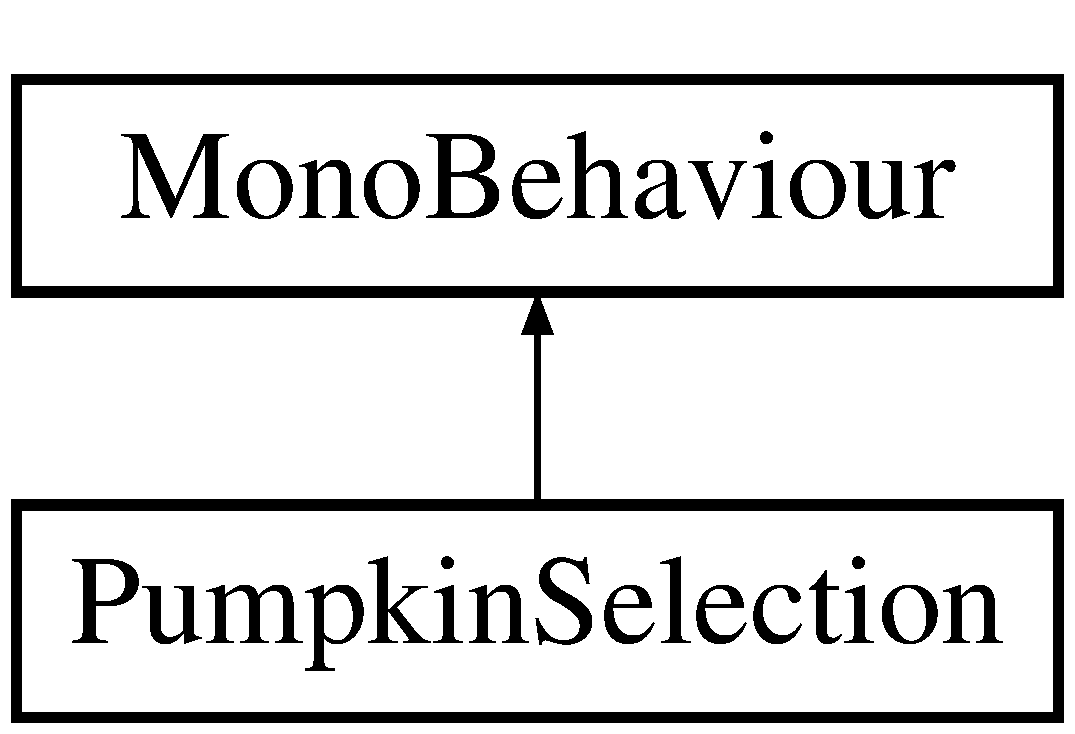
\includegraphics[height=2.000000cm]{class_pumpkin_selection}
\end{center}
\end{figure}
\subsection*{Public Attributes}
\begin{DoxyCompactItemize}
\item 
\mbox{\Hypertarget{class_pumpkin_selection_aa4c83c30a63e78ab3d69f4bf4b949be2}\label{class_pumpkin_selection_aa4c83c30a63e78ab3d69f4bf4b949be2}} 
Game\+Object {\bfseries pumpkin\+Prefab}
\end{DoxyCompactItemize}
\subsection*{Properties}
\begin{DoxyCompactItemize}
\item 
\mbox{\Hypertarget{class_pumpkin_selection_aa185d738a4c716d8dddd1b9b9be5b269}\label{class_pumpkin_selection_aa185d738a4c716d8dddd1b9b9be5b269}} 
Sprite {\bfseries Sprite}\hspace{0.3cm}{\ttfamily  \mbox{[}get\mbox{]}}
\end{DoxyCompactItemize}


\subsection{Detailed Description}
Gestioneaza dovleacul selectat 

The documentation for this class was generated from the following file\+:\begin{DoxyCompactItemize}
\item 
Halloween\+Attack/\+Assets/halloween\+Attack/\+Scripts/Pumpkin\+Selection.\+cs\end{DoxyCompactItemize}

\hypertarget{class_rotate}{}\section{Rotate Class Reference}
\label{class_rotate}\index{Rotate@{Rotate}}
Inheritance diagram for Rotate\+:\begin{figure}[H]
\begin{center}
\leavevmode
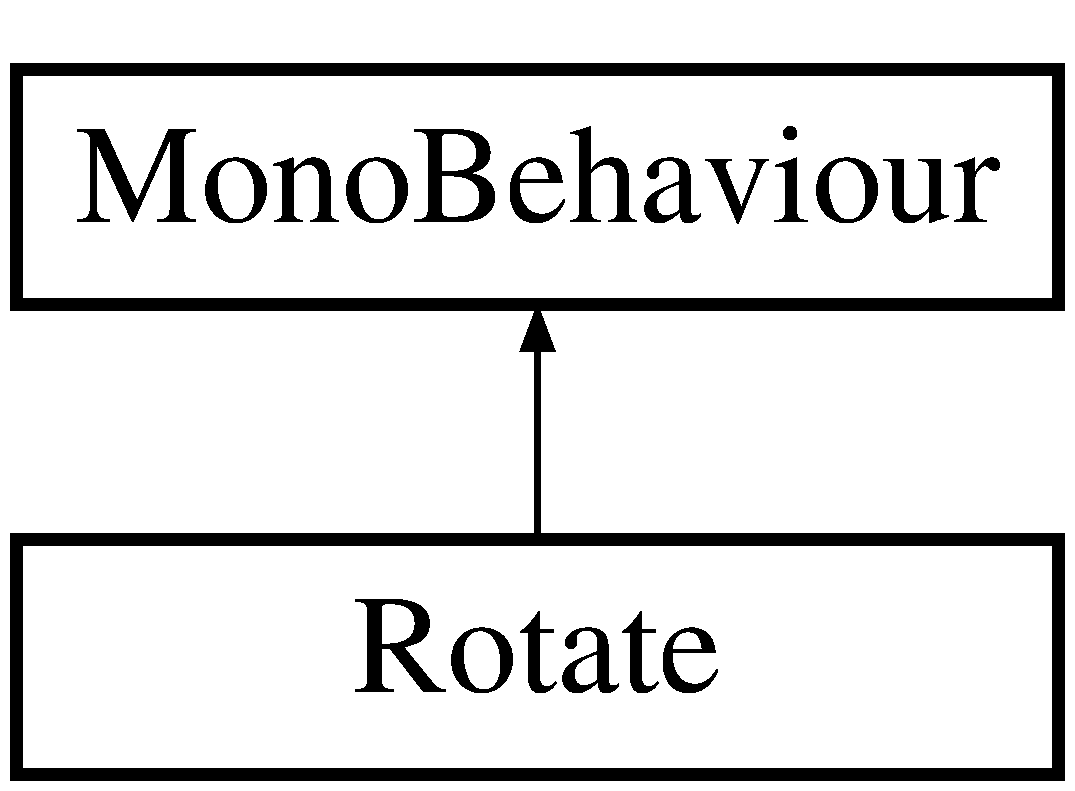
\includegraphics[height=2.000000cm]{class_rotate}
\end{center}
\end{figure}


\subsection{Detailed Description}
Se ocupa de miscarea de rotatie a dovleacului rotativ 

The documentation for this class was generated from the following file\+:\begin{DoxyCompactItemize}
\item 
Halloween\+Attack/\+Assets/halloween\+Attack/\+Scripts/Rotate.\+cs\end{DoxyCompactItemize}

\hypertarget{class_score_script}{}\section{Score\+Script Class Reference}
\label{class_score_script}\index{Score\+Script@{Score\+Script}}
Inheritance diagram for Score\+Script\+:\begin{figure}[H]
\begin{center}
\leavevmode
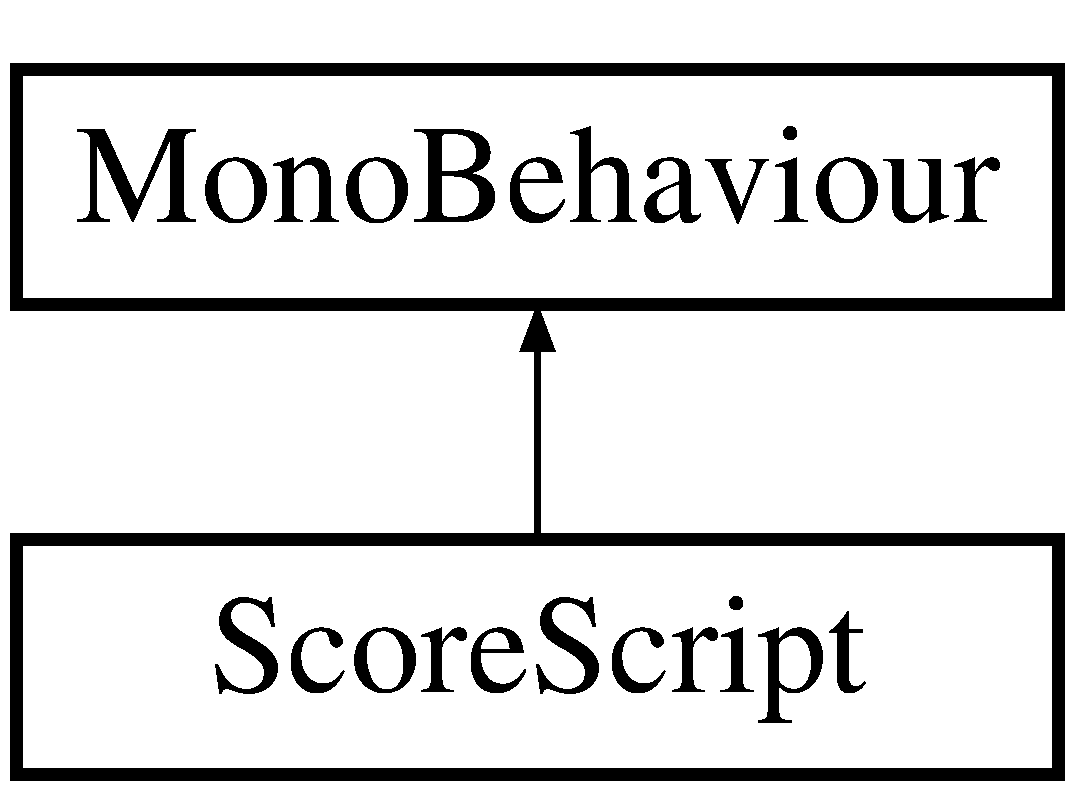
\includegraphics[height=2.000000cm]{class_score_script}
\end{center}
\end{figure}
\subsection*{Static Public Attributes}
\begin{DoxyCompactItemize}
\item 
static int \hyperlink{class_score_script_a764663ff02a695ee377080f1fecc9296}{score\+Value} = 50
\end{DoxyCompactItemize}


\subsection{Detailed Description}
Gestioneaza scorul jocului 

\subsection{Member Data Documentation}
\mbox{\Hypertarget{class_score_script_a764663ff02a695ee377080f1fecc9296}\label{class_score_script_a764663ff02a695ee377080f1fecc9296}} 
\index{Score\+Script@{Score\+Script}!score\+Value@{score\+Value}}
\index{score\+Value@{score\+Value}!Score\+Script@{Score\+Script}}
\subsubsection{\texorpdfstring{score\+Value}{scoreValue}}
{\footnotesize\ttfamily int Score\+Script.\+score\+Value = 50\hspace{0.3cm}{\ttfamily [static]}}

Scorul curent 

The documentation for this class was generated from the following file\+:\begin{DoxyCompactItemize}
\item 
Halloween\+Attack/\+Assets/halloween\+Attack/\+Scripts/Score\+Script.\+cs\end{DoxyCompactItemize}

\hypertarget{class_singleton}{}\section{Singleton$<$ T $>$ Class Template Reference}
\label{class_singleton}\index{Singleton$<$ T $>$@{Singleton$<$ T $>$}}


Be aware this will not prevent a non singleton constructor such as {\ttfamily T myT = new T();} To prevent that, add {\ttfamily protected T () \{\}} to your singleton class.  


Inheritance diagram for Singleton$<$ T $>$\+:\begin{figure}[H]
\begin{center}
\leavevmode
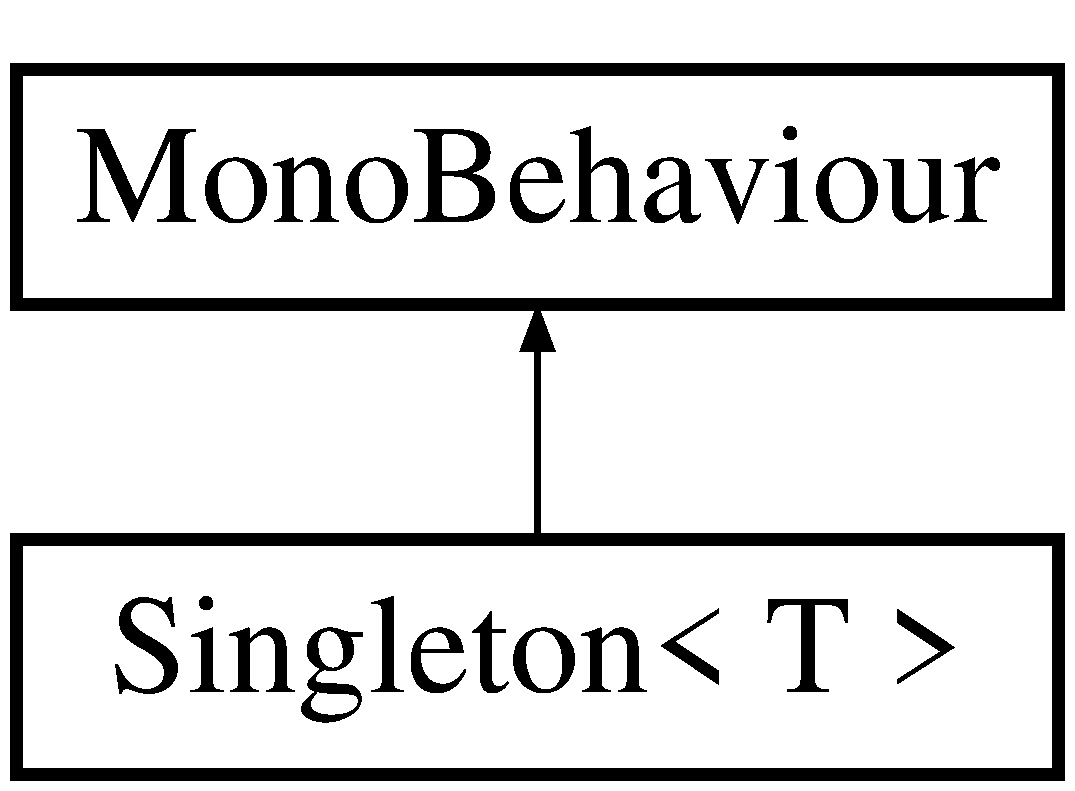
\includegraphics[height=2.000000cm]{class_singleton}
\end{center}
\end{figure}
\subsection*{Public Member Functions}
\begin{DoxyCompactItemize}
\item 
void \hyperlink{class_singleton_a81a4ea792b927aeae3f52c1e0d2036af}{On\+Destroy} ()
\begin{DoxyCompactList}\small\item\em When Unity quits, it destroys objects in a random order. In principle, a \hyperlink{class_singleton}{Singleton} is only destroyed when application quits. If any script calls Instance after it have been destroyed, it will create a buggy ghost object that will stay on the Editor scene even after stopping playing the Application. Really bad! So, this was made to be sure we\textquotesingle{}re not creating that buggy ghost object. \end{DoxyCompactList}\end{DoxyCompactItemize}
\subsection*{Properties}
\begin{DoxyCompactItemize}
\item 
\mbox{\Hypertarget{class_singleton_a54103e8475b2a352ee759d5732307534}\label{class_singleton_a54103e8475b2a352ee759d5732307534}} 
static T {\bfseries Instance}\hspace{0.3cm}{\ttfamily  \mbox{[}get\mbox{]}}
\end{DoxyCompactItemize}


\subsection{Detailed Description}
Be aware this will not prevent a non singleton constructor such as {\ttfamily T myT = new T();} To prevent that, add {\ttfamily protected T () \{\}} to your singleton class. 

As a note, this is made as Mono\+Behaviour because we need Coroutines. \begin{Desc}
\item[Type Constraints]\begin{description}
\item[{\em T} : {\em Mono\+Behaviour}]\end{description}
\end{Desc}


\subsection{Member Function Documentation}
\mbox{\Hypertarget{class_singleton_a81a4ea792b927aeae3f52c1e0d2036af}\label{class_singleton_a81a4ea792b927aeae3f52c1e0d2036af}} 
\index{Singleton@{Singleton}!On\+Destroy@{On\+Destroy}}
\index{On\+Destroy@{On\+Destroy}!Singleton@{Singleton}}
\subsubsection{\texorpdfstring{On\+Destroy()}{OnDestroy()}}
{\footnotesize\ttfamily void \hyperlink{class_singleton}{Singleton}$<$ T $>$.On\+Destroy (\begin{DoxyParamCaption}{ }\end{DoxyParamCaption})}



When Unity quits, it destroys objects in a random order. In principle, a \hyperlink{class_singleton}{Singleton} is only destroyed when application quits. If any script calls Instance after it have been destroyed, it will create a buggy ghost object that will stay on the Editor scene even after stopping playing the Application. Really bad! So, this was made to be sure we\textquotesingle{}re not creating that buggy ghost object. 



The documentation for this class was generated from the following file\+:\begin{DoxyCompactItemize}
\item 
Halloween\+Attack/\+Assets/halloween\+Attack/\+Scripts/Singleton.\+cs\end{DoxyCompactItemize}

\hypertarget{class_you_loose}{}\section{You\+Loose Class Reference}
\label{class_you_loose}\index{You\+Loose@{You\+Loose}}
Inheritance diagram for You\+Loose\+:\begin{figure}[H]
\begin{center}
\leavevmode
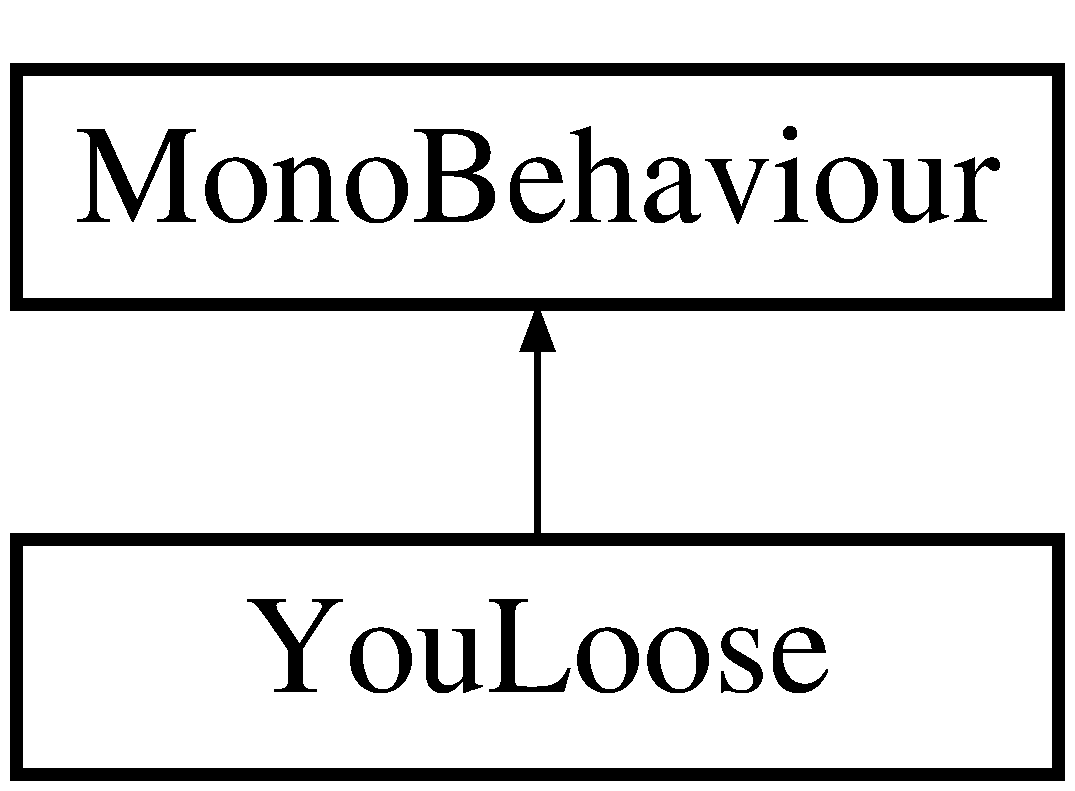
\includegraphics[height=2.000000cm]{class_you_loose}
\end{center}
\end{figure}


\subsection{Detailed Description}
Gestioneaza actiunile in momentul pierderii 

The documentation for this class was generated from the following file\+:\begin{DoxyCompactItemize}
\item 
Halloween\+Attack/\+Assets/halloween\+Attack/\+Scripts/You\+Loose.\+cs\end{DoxyCompactItemize}

%--- End generated contents ---

% Index
\backmatter
\newpage
\phantomsection
\clearemptydoublepage
\addcontentsline{toc}{chapter}{Index}
\printindex

\end{document}
